\begin{frame}
  \frametitle{Structures of Schottky Diodes}
  2 structures of the schottky diodes are finding wide applications:
  \begin{itemize}
  \item Microwave detection and mixing
  \item Integrated circuits
  \end{itemize}
\end{frame}

\begin{frame}
  \begin{figure}[h]
    \caption{Small area Microwave Schottky diode detector}
    \centering
    \includegraphics[width=0.5\textwidth]{./images/chapter8/fig8_6.png}
    \label{fig:8_6}
  \end{figure}
  A small area semiconductor diode formed by depositing metal by planar process on an epitaxail or $n^+$ substrate is used. The series resistance and the diode capacitance have to be minimized for good performance. The cut-off frequency for forward bias is given by:
  $f_c = \frac{1}{2\pi R_{f}C_f}$ where $R_f$ and $C_f$ are values for forward bias of 0.1 V
\end{frame}
\begin{frame}
  \begin{figure}[h]
    \caption{Metal overlap Schottky structure}
    \centering
    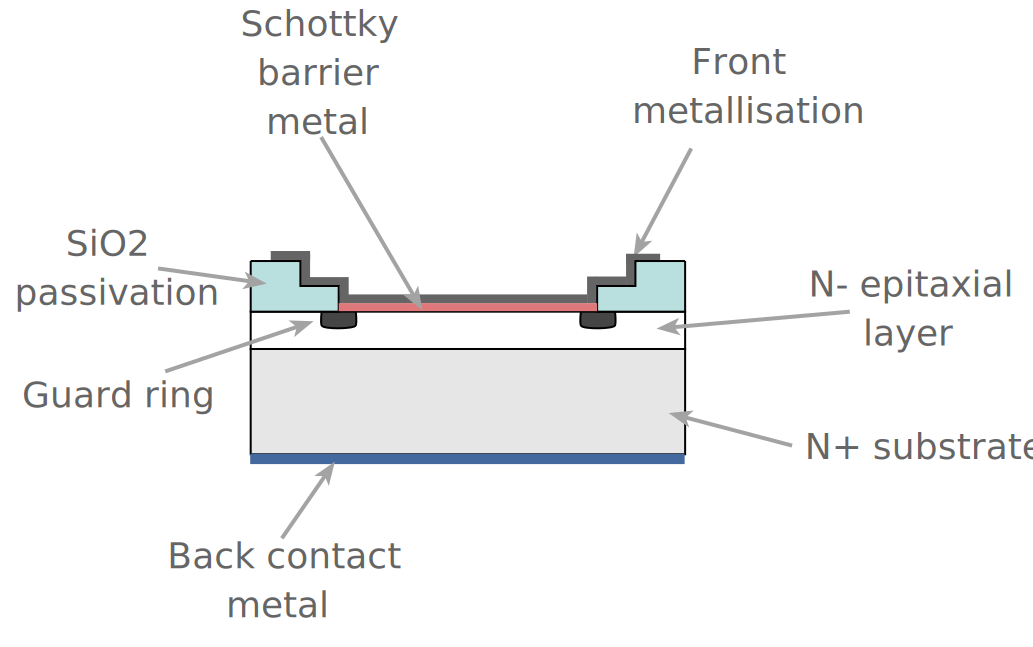
\includegraphics[width=0.4\textwidth]{./images/chapter8/fig8_8.png}
    \label{fig:8_8}
  \end{figure}
  This structure is well suited for integrated circuits. It gives a well forward I-V characteristic and low leakage current. The metal semiconductor junction will behave as an ohmic contact when the semiconductoris highly doped. The heavily doped surface can be formed by shallow diffusion or alloy regrowth.
\end{frame}

\begin{frame}
  The heavily doped layer in the metal semiconductor junction leads to extremely thin a depletion layer. The carriers can tunnel easily through this thin depletion layer from semiconductor to metal and the diffusion of the carriers can tunnel easily through this thin depletion layer from semiconductor to metal and the diffusion of the carriers over the contact potential plays a minor role.  Thus current flows through tunnelling of the electrons from the semiconductor to the metal irrespective of the polarity of the bias voltage. Thus current can flow in both the directions making the metal semiconductor junction behave like an ohmic contact.

\end{frame}